
%\documentclass[mathserif]{beamer}
\documentclass[handout]{beamer}
%\usetheme{Goettingen}
%\usetheme{Warsaw}
\usetheme{Singapore}



%\usetheme{Frankfurt}
%\usetheme{Copenhagen}
%\usetheme{Szeged}
%\usetheme{Montpellier}
%\usetheme{CambridgeUS}
%\usecolortheme{}
%\setbeamercovered{transparent}
\usepackage[english, activeacute]{babel}
\usepackage[utf8]{inputenc}
\usepackage{amsmath, amssymb}
\usepackage{dsfont}
\usepackage{graphics}
\usepackage{cases}
\usepackage{graphicx}
\usepackage{pgf}
\usepackage{epsfig}
\usepackage{amssymb}
\usepackage{multirow}	
\usepackage{amstext}
\usepackage[ruled,vlined,lined]{algorithm2e}
\usepackage{amsmath}
\usepackage{epic}
\usepackage{epsfig}
\usepackage{fontenc}
\usepackage{framed,color}
\usepackage{palatino, url, multicol}
%\algsetup{indent=2em}
\newcommand{\factorial}{\ensuremath{\mbox{\sc Factorial}}}
\newcommand{\BIGOP}[1]{\mathop{\mathchoice%
{\raise-0.22em\hbox{\huge $#1$}}%
{\raise-0.05em\hbox{\Large $#1$}}{\hbox{\large $#1$}}{#1}}}
\newcommand{\bigtimes}{\BIGOP{\times}}
\vspace{-0.5cm}
\title{Natural Language Processing \\ Recursive Networks and Paragraph Vectors}
\vspace{-0.5cm}
\author[Felipe Bravo Márquez]{\footnotesize
%\author{\footnotesize  
 \textcolor[rgb]{0.00,0.00,1.00}{Felipe Bravo-Marquez}} 
  
 

\date{\today}

\begin{document}
\begin{frame}
\titlepage


\end{frame}


\begin{frame}{Recursive Neural Networks over Sentiment Treebank}
\begin{scriptsize}
\begin{itemize}
\item A recursive neural tensor network for learning the sentiment of pieces of texts of different granularities, such as words, phrases, and sentences, was proposed in~\cite{socher2013recursive}.
\item The network was trained on a sentiment annotated treebank \url{http://nlp.stanford.edu/sentiment/treebank.html} of parsed sentences for learning compositional vectors of words and phrases.
\item Every node in the parse tree receives a vector, and there is a matrix capturing how the meaning of adjacent nodes changes. 
\item The network is trained using a variation of backpropagation called Backprop through Structure.
\item The main drawback of this model is that it relies on parsing.
\end{itemize}
\end{scriptsize}
\end{frame}


\begin{frame}{Recursive Neural Networks over Sentiment Treebank}
   
    \begin{figure}[h]
        	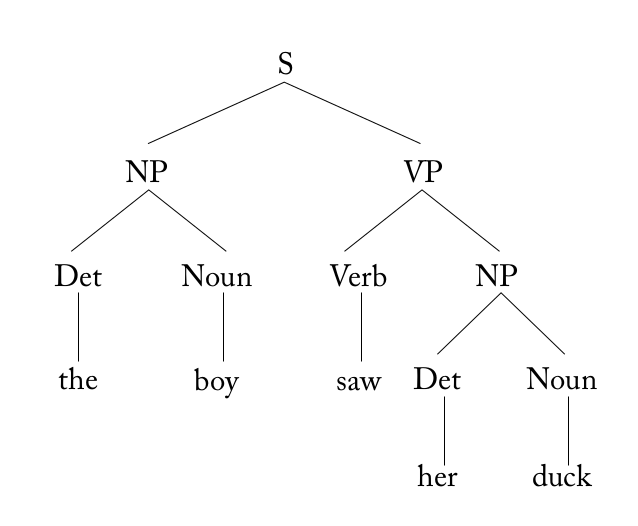
\includegraphics[scale = 0.45]{pics/parseTree.png}
        	\caption{A parse tree}
        \end{figure}       
        
\end{frame}





\begin{frame}{Recursive Neural Networks over Sentiment Treebank}
   
    \begin{figure}[h]
        	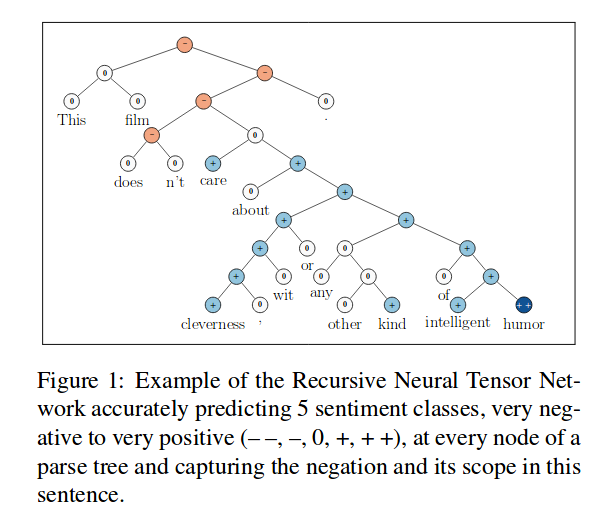
\includegraphics[scale = 0.45]{pics/recTensor1.png}
        \end{figure}       
        
\end{frame}


\begin{frame}{Recursive Neural Networks over Sentiment Treebank}
   
    \begin{figure}[h]
        	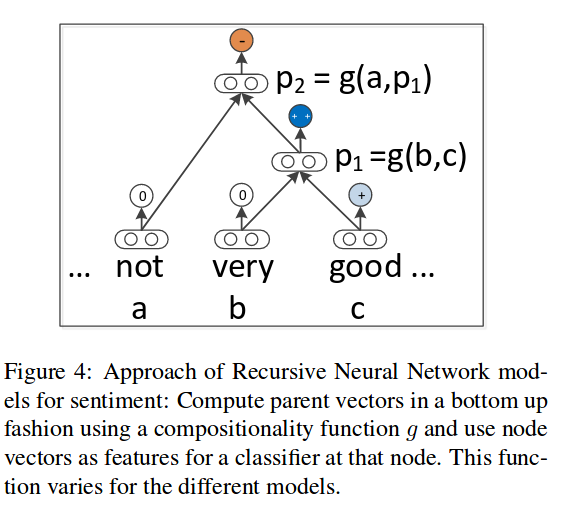
\includegraphics[scale = 0.45]{pics/recTensor2.png}
        \end{figure}       
        
\end{frame}



\begin{frame}{Paragraph vector}
% See dissapointment slide http://videolectures.net/deeplearning2015_manning_deep_learning/
\begin{scriptsize}
\begin{itemize}
\item A paragraph vector-embedding model that learns vectors for sequences of words of arbitrary length (e.g, sentences, paragraphs, or documents) without relying on parsing was proposed in~\cite{LeM14}. 
\item The paragraph vectors are obtained by training a similar network as the one used for training the CBOW embeddings. 
\item The words surrounding a centre word in a window are used as input together with a paragraph-level vector for predict the centre word. 
\item The paragraph-vector acts as a memory token that is used for all the centre words in the paragraph during the training the phase. 
\item The recursive neural tensor network and the paragraph-vector embedding were evaluated on the same movie review dataset used in \cite{Pang2002}, obtaining an accuracy of 85.4\% and 87.8\%, respectively. 
\item Both models outperformed the results obtained by classifiers trained on representations based on bag-of-words features.
\item Many researchers have have  struggled  to  reproduce these paragraph vectors \cite{lau2016empirical}.  
\end{itemize}
\end{scriptsize}
\end{frame}


\begin{frame}{Paragraph vector}
   
    \begin{figure}[h]
        	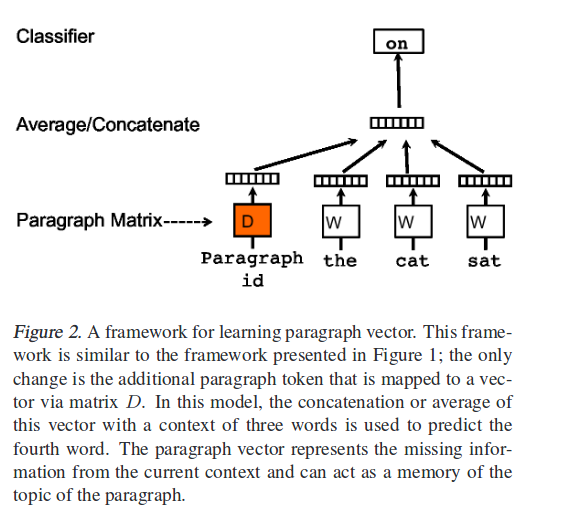
\includegraphics[scale = 0.45]{pics/doc2vec.png}
        \end{figure}       
        
\end{frame}


\begin{frame}{Summary}
\begin{scriptsize}
\begin{itemize}
\item Neural networks are making improvements across many NLP tasks (e.g., sentiment analysis, machine translation).
\item Deep Learning $!=$ Feature Engineering.
\item Word embeddings provide a practical framework for semi-supervised learning (i.e., leveraging unlabeled data).
\item Character-level embeddings are worth paying attention to!
\item Convolutional neural networks can capture useful features (e.g., n-grams) regardless of the position.
\item Recurrent Neural Networks are very useful for learning temporal patterns, especially for long dependencies.
\item We just scratched the surface!!
\end{itemize}
\end{scriptsize}
\end{frame}




\begin{frame}
\frametitle{Questions?}
%\vspace{1.5cm}
\begin{center}\LARGE Thanks for your Attention!\\ \end{center}



\end{frame}

\begin{frame}[allowframebreaks]\scriptsize
\frametitle{References}
\bibliography{bio}
\bibliographystyle{apalike}
%\bibliographystyle{flexbib}
\end{frame}  


%%%%%%%%%%%%%%%%%%%%%%%%%%%

\end{document}
